\documentclass{article}
\usepackage[utf8]{inputenc}
\usepackage{amssymb}
\usepackage{mathtools} 
\usepackage{geometry}
 \geometry{
 a4paper,
 total={140mm,227mm},
 left=35mm,
 top=35mm,
 }

\usepackage{float}
\usepackage{graphicx}
\usepackage{epstopdf}
\usepackage{amsmath}
\usepackage{bm}

\setlength{\parindent}{0pt}
\numberwithin{figure}{section}
% equation number format: in section 1, (1.1), (1.2) ..
\usepackage{amsmath}
\numberwithin{equation}{section}

\makeatletter
% we use \prefix@<level> only if it is defined
\renewcommand{\@seccntformat}[1]{%
  \ifcsname prefix@#1\endcsname
    \csname prefix@#1\endcsname
  \else
    \csname the#1\endcsname\quad
  \fi}
% define \prefix@section
% \newcommand\prefix@section{}
\makeatother

%% multi col
\usepackage{multicol}

% hyperlinks
\usepackage{hyperref}
\hypersetup{
    colorlinks=true,
    linkcolor=black,   
    urlcolor=black,
    filecolor=black,
} 
\urlstyle{same}

% colored frames (boxes)
\usepackage{xcolor}
\usepackage{mdframed}

% vector arrow with \vv{ }
\usepackage{esvect}

%\hyphenpenalty 10000
%\exhyphenpenalty 10000
%\usepackage[none]{hyphenat}
%\usepackage[document]{ragged2e}

% strike through text
\usepackage[normalem]{ulem}
% \sout{Hello World}

%%%%%%%%%%%%%%%%%%
%% HEADER OVER %%%
%%%%%%%%%%%%%%%%%%

\usepackage{listings}
\lstset{language=C,
basicstyle=\ttfamily,
keywordstyle=\color{blue}\ttfamily,
stringstyle=\color{red}\ttfamily,
commentstyle=\color{green}\ttfamily,
morecomment=[l][\color{magenta}]{\#}, 
numbers=left,
numbersep=5pt, 
backgroundcolor=\color{white}, 
breaklines=true
}

\usepackage{siunitx}

\title{02131 Assignment 1 \\Software implementation of a personal ECG scanner}
\author{s144107 Roar Nind Steffensen\\s144063 Magnus Søborg-Madsen}
\date{2016-09-26}

\begin{document}
%\maketitle

\begin{titlepage}
\centering
\parindent=0pt
\newcommand{\HRule}{\rule{\textwidth}{1mm}}
 \HRule\\[1cm]\huge\textbf
{02131 Assignment 1 \\Software implementation of a personal ECG scanner}\\[0.1cm]
\HRule\\[3cm]\vspace{-1 cm} \textbf{\Large{group RR \& MGNS}}\\
\large{
Roar Nind Steffensen (s144107)\\
Magnus Middelboe Søborg-Madsen (s144063)}

\vspace{2 cm}

\vspace{0.5cm}
\begin{figure}[h]
\centering
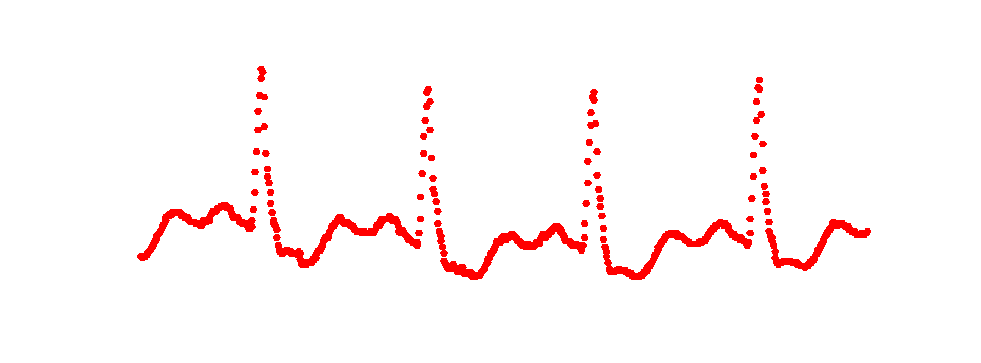
\includegraphics[width=1.0\textwidth]{frontpage/frontpage.eps}
\label{fig:front}
\end{figure}

\vspace*{\stretch{2}} \normalsize %
Technical University of Denmark\\
29 Sep 2016
%\vspace*{-1cm}
\begin{figure}[h]
    \centering
    
\includegraphics[height=2cm]{frontpage/DTUlogo.png}
\end{figure}
\end{titlepage}

%\begin{figure}[H]
%\centering
%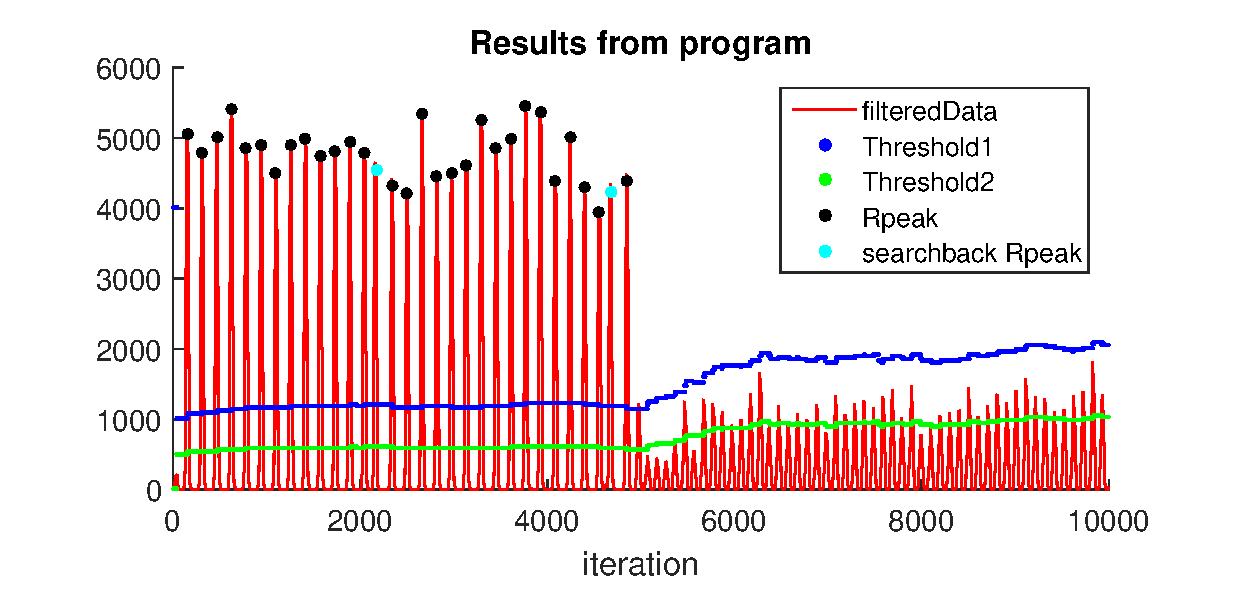
\includegraphics[width=1.0\textwidth]{3Results/fig/10kpointsmatlab.eps}
%\label{fig:front}
%\end{figure}

\newpage
\setcounter{tocdepth}{2}

\tableofcontents
\vfill
\section*{Responsibility chart}
\begin{multicols}{2}

\begin{table}[H]
\centering
\begin{tabular}{ll}
\textbf{C code}         & \textbf{resp.} \\
coding C                & both       \\
main.c                  & both       \\
filters.c               & both       \\
qsr.c                   & both       \\
peak detection          & R          \\
searchback              & both       \\
comments in .c and .h files                                                    & both       \\
Eclipse, fedora         & both          \\
loading/writing to files & R          \\
optimization: pass by ref                                                      & both       \\
shiftarray, printarray  & both       \\
performance test        & R          \\
                        &           \\
\textbf{Meetings}       & \textbf{resp.}\\
Bringing food           & both  
\end{tabular}
\end{table}


\begin{table}[H]
\centering
\begin{tabular}{ll}
\textbf{Report}         & \textbf{resp}. \\
Introduction            & M     \\
Design: data            & both  \\
Design: filters         & M     \\
Design: filters in C    & both     \\
QRS algorithm: peak detection                                                  & both  \\
Impl.: overall structure & both  \\
Impl.: Data types       & M     \\
Impl.: Start and end    & R     \\
Results: plots, text    & both  \\
Results: plots MATLAB   & M     \\
Performance test        & R     \\
Conclusion              & both  \\
Appendix A: Filter      & both  \\
Appendix B: struct      & M    
\end{tabular}
\end{table}

\end{multicols}

\vspace{1 cm}

\newpage
\section{Introduction}
In the DTU course \texttt{02131 Embedded Systems}, we pretend to be engineers at the fictive company \texttt{Medembed}. Our task is to investigate whether the Pan-Thompkins QRS detection algorithm can be used in a personal wearable ECG (\underline{e}lectro\underline{c}ardio\underline{g}ram) scanner. In this report, we document how we implemented the QRS algorithm in C, and determine whether the algorithm can be implemented reasonably in an embedded system.

\section{Design}
\subsection{Data}
In the real world, data from a personal ECG scanner is acquired continuously, one data point at a time. As a consequence, our program must be able to continuously acquire, filter, and process data. In order to show warnings in real time, the program must process data faster than it is acquired. \\ We simulated this by reading data points one-by-one, from a \texttt{.txt} file containing signal amplitudes. The data points are stored in a 33-point \color{blue} \texttt{int} \color{black} array called \texttt{originalArray} located in a struct called \texttt{data}. All values in \texttt{originalArray} are initialized to 0. With these initial values, the first $\approx$ 30 filtered data points are calculated using zeros, so with a sample rate of 250 Hz, the data acquisition causes a $\frac{30}{250 \, \si{Hz}} =$ 12 ms startup delay. The rewritten code below summarizes our data acquisition.


\begin{lstlisting}
 FILE* file = fopen("ECG.txt", "r"); // File pointer for input from file
while(fscanf(file, "%i", &(data.originalArray[ARRAY_LENGTH - 1])) != EOF){
        // body of main loop
        ...
        }
\end{lstlisting}

The loop header attempts to read a new data point, and if it succeeds (we're not at the end of the \texttt{.txt} file), the loop is executed. The bulk of the program execution happens within this \color{blue} \texttt{while} \color{black} loop: For each new data point acquired, the functions handling filtering and peak detection are called. The data points are sent to filters using \textbf{pass by reference}.
%  Hvordan opsamles og gemmes data til filtrene



\subsection{Filters}
In \texttt{filters.c}, five filters are applied: low-pass, high-pass, derivative, squaring, and moving window integration. In the following section, we present the filter equation, the purpose of the filters, and how we translated the equations to functions in \texttt{C}. 

\subsubsection{Low-pass filter}
If we reconstruct the signal using sine waves (Fourier series), we can choose to filter out sine waves with frequencies too high or too low to reasonably represent a QRS complex. The low-pass filter used has a cutoff frequency of $\approx$ 12 Hz, and is represented by the following difference equation:

\begin{equation}
    y_n = 2y_{n-1} - y_{n-2} + \frac{1}{32} \cdot (x_n - 2x_{n-6} + x_{n-12})
\end{equation}

\subsubsection{High-pass}
The high-pass filter used has a cutoff frequency of $\approx$ 6 Hz, and is represented by the difference equation below. After the data has been through the low-pass and high-pass filters, the remaining signal (in the frequency domain) is centered around 5-20 Hz due to the continuous cutoffs. 
\begin{equation}
    y_n = y_{n-1} -\frac{x_n}{32} + x_{n-16} - x_{n-17} + \frac{x_{n-32}}{32}
\end{equation}

\subsubsection{Derivative}
Now the signal is differentiated, since we are interested in the slope, and most importantly: when the peak (maximum) occurs in the time-domain. 
\begin{equation}
    y_n = \frac{1}{8} \cdot (2x_n + x_{n-1} - x_{n-3} - 2x_{n-4} )
\end{equation}

\subsubsection{Squaring}
Now all values are squared to emphasize large differences in the original data, and to make all values positive.
\begin{equation}
    y_n = x_n^2
\end{equation}

\subsubsection{Moving window integration}
Finally the signal is integrated over the past $N = 30$ signal values. This is achieved by the difference equation below:
\begin{equation}
    y_n = \frac{1}{N} (x_{n- (N-1)}  + x_{n-(N-2)} + ... +  x_n )
\end{equation}

By differentiating, squaring, and then integrating, the filtered data signal is comparable to the original signal; the values represent an amplitude (as a function of time). Each filter causes a delay, e.g. we only obtain the final filtered data point $y_n$ after applying the last filter to the previous 30 data points. See Appendix \eqref{Apx:A} to see how the filters alter the original signal.

\subsubsection{Filters in C}
The function \texttt{filterData} in \texttt{main.c} calls the filter functions in the correct order, by passing memory addresses to arrays, and an int representing the array length. \\
\\
We combined the derivative and squaring filters, and added a function that shifts the array, similar to the \texttt{HackerRank} rotating circular array exercise. After an array has been shifted, the penultimate and ultimate values are identical, so the array is ready for a new value. The following code summarizes how we invoke the filtering in \texttt{main.c}:

\begin{lstlisting}
void filterData(DATA *data){
    shiftArray(data->afterLowPass, ARRAY_LENGTH);
    // applies low pass filter
    data->afterLowPass[ARRAY_LENGTH-1] = lowPassFilter(data->afterLowPass, data->originalArray, ARRAY_LENGTH);
...}
\end{lstlisting}

\texttt{data} is the struct containing all relevant variables: integers, doubles, arrays. The arrays are named after which filter has been applied most recently.
filterData is of type void; it only calls the other filter functions. The filter functions are kept as close to the template as possible, e.g. compare the low pass filter equation with the function \texttt{lowPassFilter}:

\begin{equation}
    y_n = 2 y_{n-1} - y_{n-2} + (x_n + 2x_{n-6}+ x_n{-12})/32
\end{equation}

\begin{lstlisting}
int lowPassFilter(int * y, int * x, int n){
    return 2*y[n-1] - y[n-2] + (x[n] - 2*x[n-6] + x[n-12])/32;
}
\end{lstlisting}


\subsection{QRS algorithm: peak detection}
\label{sx:QRSalg}
Peak detection is invoked with a single function call in \texttt{main.c}. We implemented the algorithm similar to the template, with certain differences. All variables used in peak detection are stored in the struct \texttt{data}. \texttt{data} contains all used variables and arrays of length 33: filtered data, Rpeaks etc. The term "Rpeak" originates from the QRS complex\footnote{QRS complex described in "02131 Assignment 1: Software implementation of a personal ECG scanner"}, used to describe the profile of a heartbeat in a signal vs time plot. The "R" is the point for the main heartbeat with the largest amplitude, hence we use "Rpeak" for the main peak of interest.\\
\\
The algorithm is implemented in \texttt{qsr.c} in five functions, and the control flow resembles the template, see Fig \ref{fig:QRS_flowchart}. All tests (\color{blue} \texttt{if} \color{black} statements) are carried out by the function preceding the test.
% Hvordan er algoritmen implementeret og hvordan gemmes relevant data (R-peak)

\begin{figure}[H]
    \centering
    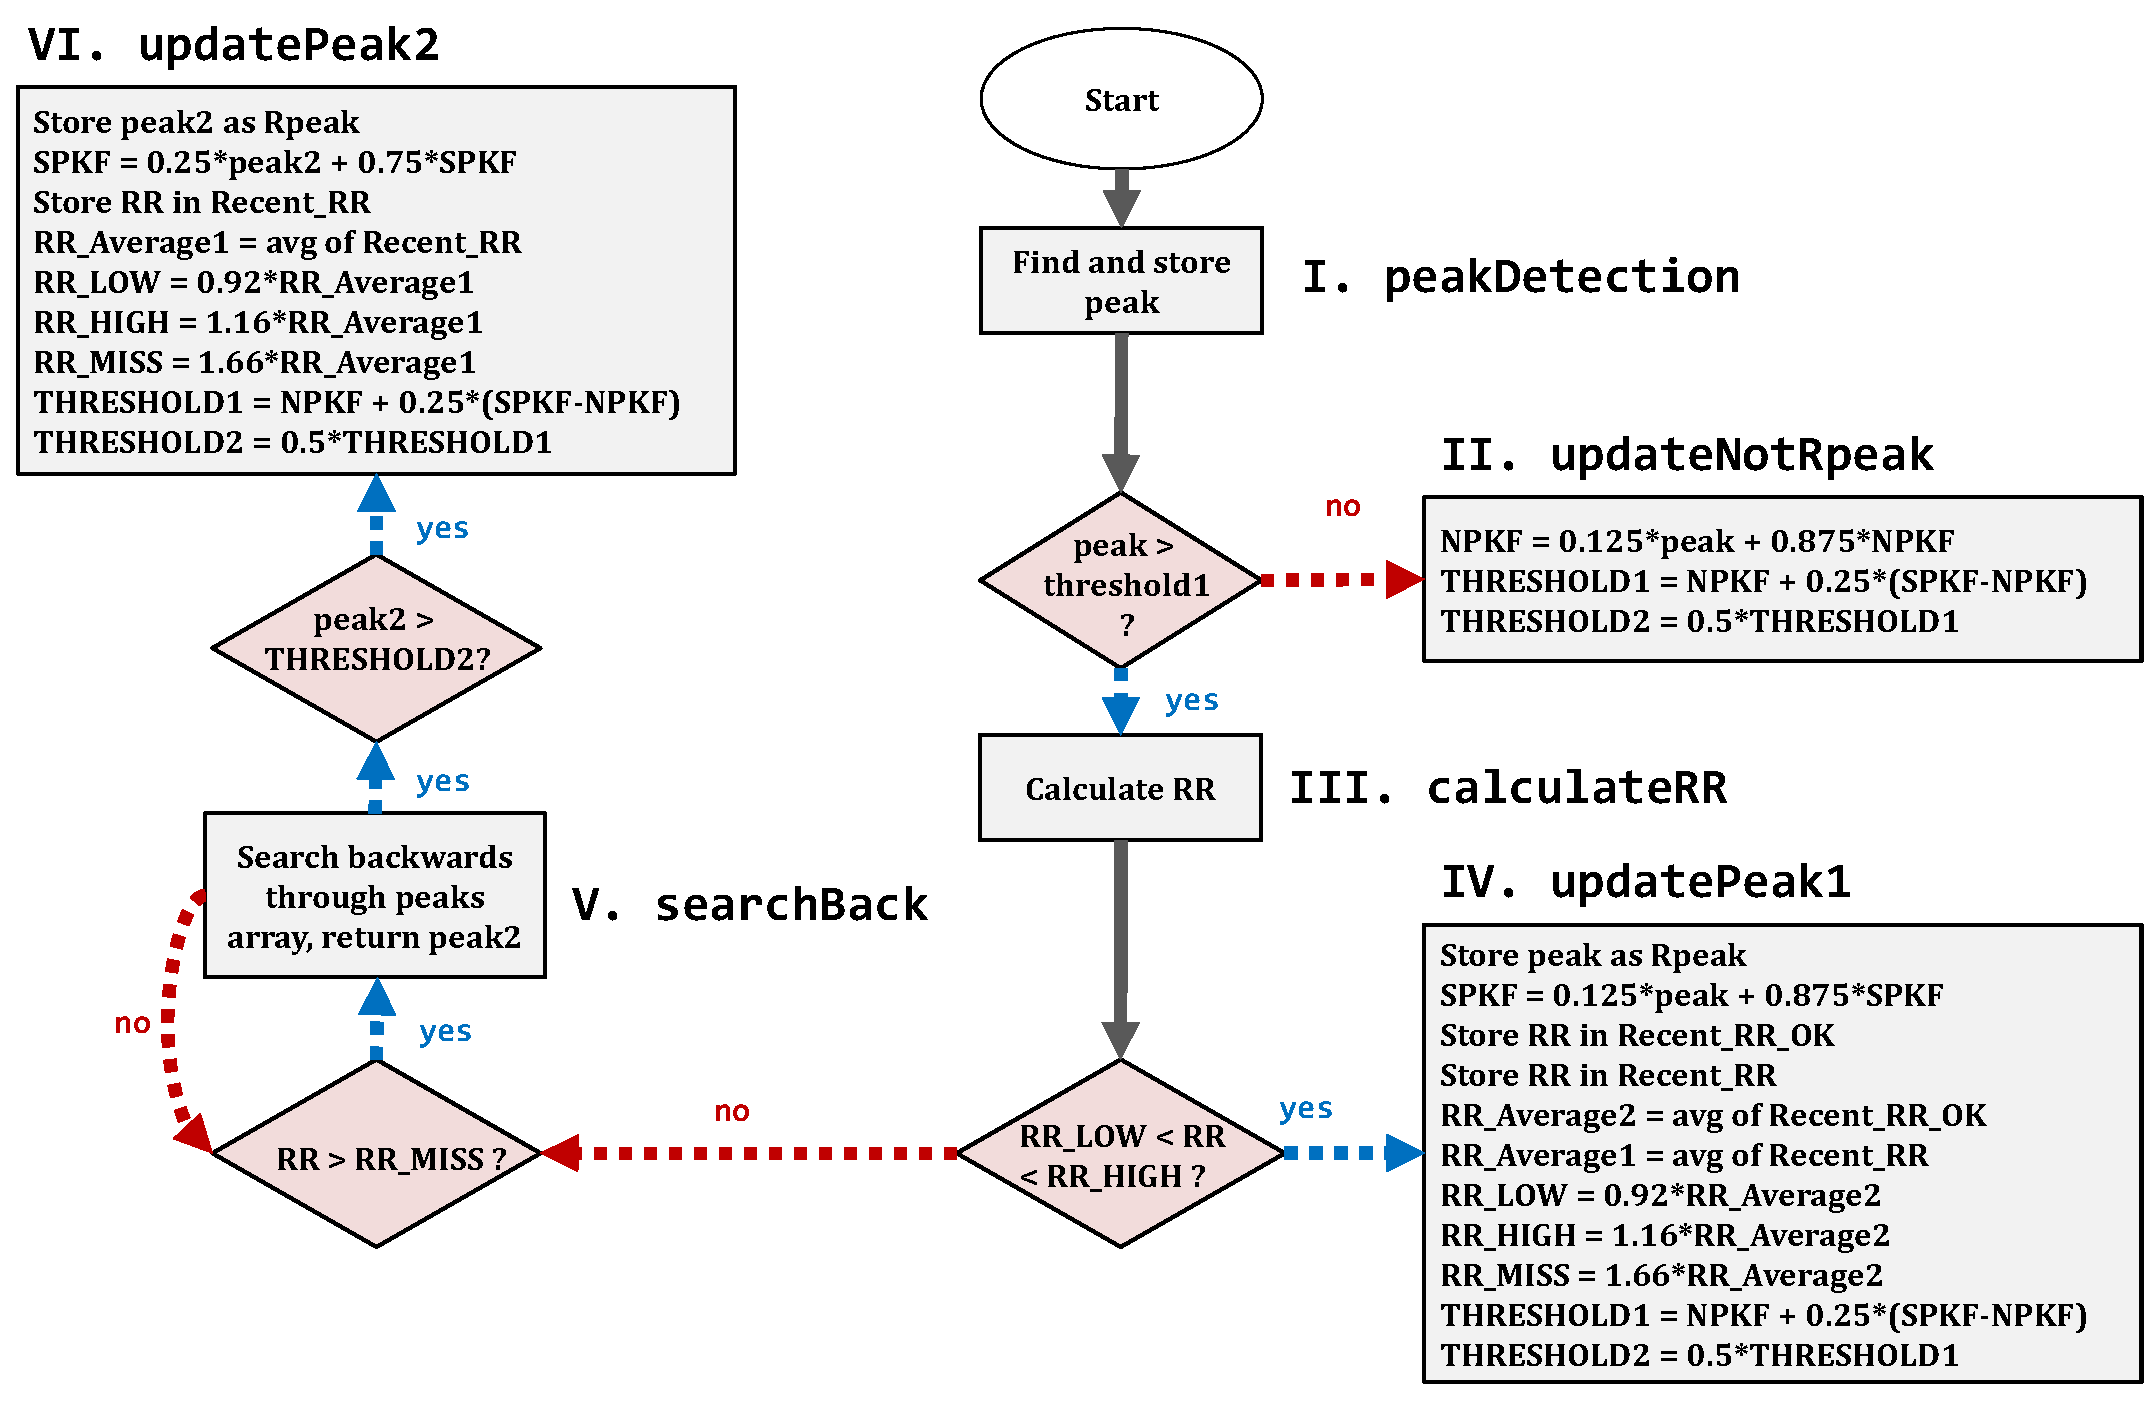
\includegraphics[width=1.0\textwidth]{1Design/fig/QRS.pdf}
    \caption{QRS algorithm flow chart, with our 6 \texttt{qrs.c} functions marked.}
    \label{fig:QRS_flowchart}
\end{figure}

In the numerated sections below, it is described how the QRS algorithm shown in figure \ref{fig:QRS_flowchart} is implemented, and how relevant data is saved for later use (e.g. R-peaks):

\subsubsection*{I. Peak detection}
In order to determine whether a peak has occurred, the last four data points ($x_n, x_{n-1}, x_{n-2}$ and $x_{n-3}$) are analyzed. For a peak to be approved as an Rpeak, the four data point must follow the pattern shown in equation \ref{eq:peakDetection}.

\begin{equation} \label{eq:peakDetection}
    x_{n-3} < x_{n-2} \geq x_{n-1} > x_n
\end{equation}

This pattern is also shown in figure \ref{fig:peakDetection} with $n-1$ being data point $x_{n-1}$ and so forth.

\begin{figure}[H]
    \centering
            
        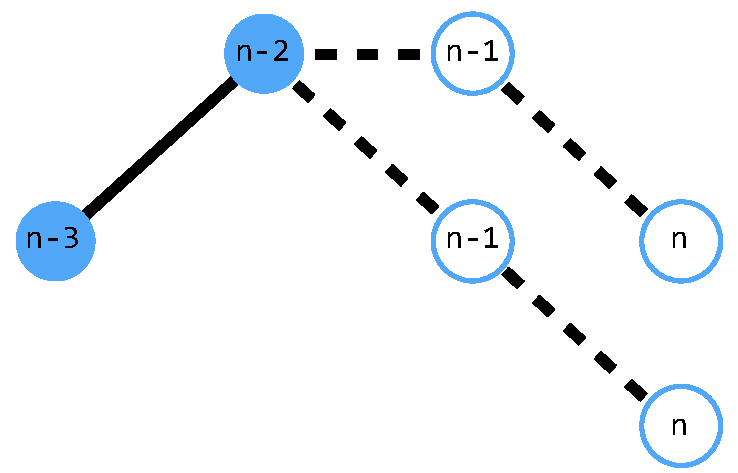
\includegraphics[width = 0.5\textwidth]{1Design/fig/peakReference.pdf}
        \caption{Peak blueprint. Straight lines symbolize a necessary relationship between data points. Dashed lines symbolize sufficient relationships between data points.}
        \label{fig:peakDetection}
\end{figure}

As seen on figure \ref{fig:peakDetection} we accept two different cases. Peaks with either one data point, or two data points at the top (a plateau). The subsequent data point must have a lower value. With this peak blueprint, the function \texttt{searchback} is only called twice during the test data: \texttt{ECG.txt}.

\subsubsection*{II. Update values: Not Rpeak}
If the peak satisfies the blueprint, but is weaker than \texttt{THRESHOLD1} (main threshold for peak amplitudes; used to discard peaks caused by noise), the peak is not saved as an Rpeak, but \texttt{THRESHOLD1} is updated accordingly. 

\subsubsection*{III. Calculate RR}
Once an accepted peak is stronger than \texttt{THRESHOLD1}, the interval between the current peak and previous Rpeak is calculated, also known as the the RR interval. This calculation uses a variable named \texttt{lastPeak} which keeps track of the iterations since last Rpeak. 

If the RR interval is between \texttt{RR\_LOW} and \texttt{RR\_HIGH} (variables to keep track of pulse rhythm) the function \texttt{updatePeak1} is called to save valid data. If the RR interval is not between these variables, the function \texttt{searchback} is called to investigate whether an Rpeak has been overlooked.

\subsubsection*{IV. Update values: peak1}
This function saves the peak as an Rpeak and adjusts variables tracking amplitude and rhythm to determine whether the patient has a stable heartbeat. This variable adjustment gives the program enough flexibility to handle the variations in the heartbeat caused by e.g. exercise and sleep.

\subsubsection*{V. Search backwards}
The \texttt{searchback} function is called if an irregularity in rhythm has occurred, and the RR interval is larger than the \texttt{RR\_MISS} variable. This suggests that an Rpeak is missed, forcing the program to look through previous peaks checking if a peak is stronger than \texttt{THRESHOLD2} (half the magnitude of \texttt{THRESHOLD1}), and if so, saving the peak as \texttt{peak2}.\\

The RR interval and \texttt{lastPeak} are adjusted according to the time between the last Rpeak and \texttt{peak2}.

\subsubsection*{VI. Update values: peak2}
Once a peak is found and stored as \texttt{peak2}, \texttt{updatePeak2} saves \texttt{peak2} as an Rpeak. This function is similar to \texttt{updatePeak1}, but instead of adjusting \texttt{RR\_LOW}, \texttt{RR\_HIGH} and \texttt{RR\_MISS} with respect to \texttt{RecentRR\_OK}, \texttt{updatePeak2} adjusts with respect to \texttt{RecentRR}. This way data from \texttt{searchback} is taken into account. See figure \ref{fig:QRS_flowchart}.

\subsection{Output}
If the heart rhythm is unstable, \texttt{qsr.c} prints a warning: "WEAK HEARTBEAT" if the R-peak value is less than 2000; "UNSTABLE RHYTHM" if 5 successive RR-intervals have missed the \texttt{RR\_LOW} and \texttt{RR\_HIGH}. \\
\\
Notice that this warning is triggered by e.g. 5 quick peaks in a row, or 5 slow peaks in a row, but also if the peak-to-peak distance alternates: quick, quick, slow, quick, slow. Hence the term \textit{unsteady} is well chosen.\\
\\
The data regularly presented to the user (not warnings) is peak amplitude, current time peak was detected and the current heart rate (BPM):\\
\\
\textbf{Peak amplitude} is the signal intensity for the given Rpeak. \\
\textbf{Current time} is calculated using how long the program has run (iterations), and the frequency of the sensor. \\
\textbf{BPM} is found using the frequency of the sensor, \texttt{RR\_AVERAGE1} for average heart rate, and converting to minutes instead of seconds. If no new Rpeak is found, BPM is set to zero. 

\section{Implementation}
\subsection{Overall program structure}
The control flow starts in \texttt{main.c} as usual, and data acquisition happens in \texttt{main.c}. As previously mentioned, all arrays with data (\texttt{afterLowPass}, \texttt{filteredData}..) are stored in a struct called \texttt{data}. When the data is filtered, \texttt{main} calls the filter functions in \texttt{filters.c}; the filter functions return integers that \texttt{main} then stores in \texttt{data}. \\
\\
In contrast, peak detection is invoked by \texttt{main} through the void function \texttt{peakDetection}. In \texttt{qsr.c}, \texttt{peakDetection} begins the chain of functions that carry out the QRS algorithm outlined in chapter \ref{sx:QRSalg}. These function directly alter the variables in \texttt{data}: the doubles \texttt{THRESHOLD1} and \texttt{THRESHOLD2}, the array \texttt{RecentRR} etc. \\
\\
User input is kept at a minimum, but \texttt{qsr.c} invokes several warnings, as outlined in the \textit{Output} chapter. 

\begin{figure}[H]
    \centering
    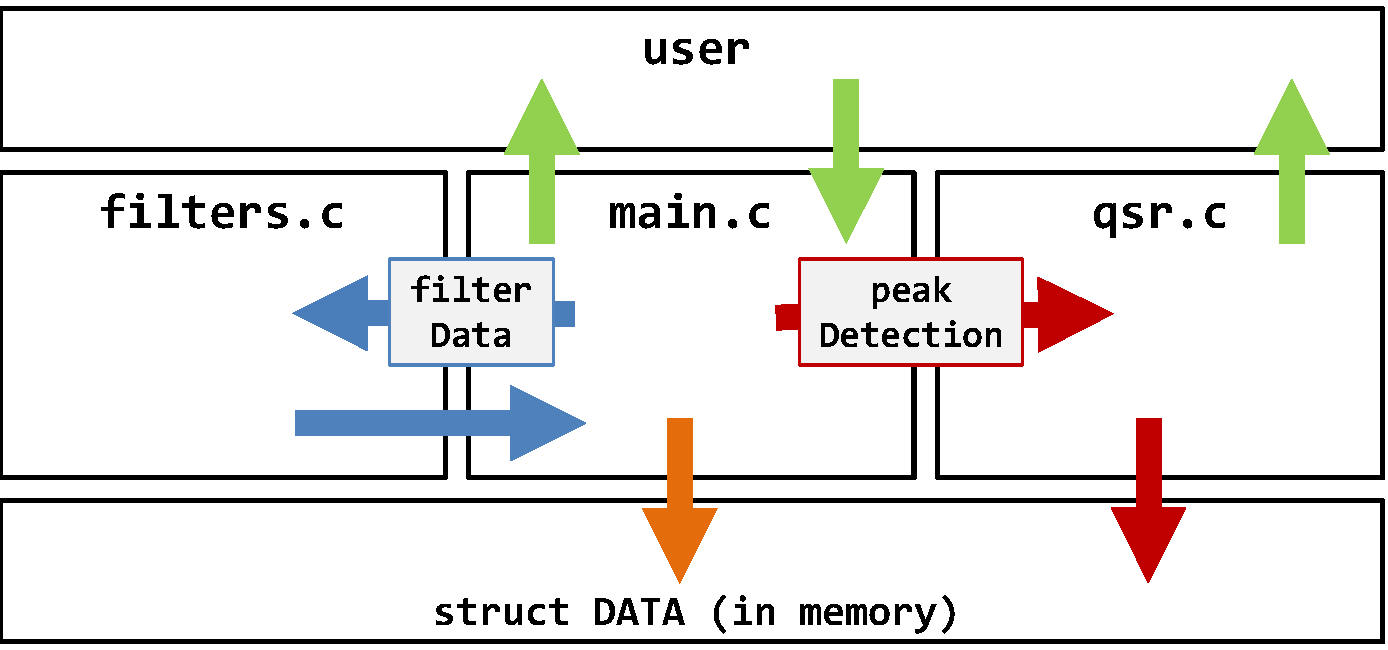
\includegraphics[width=1.0\textwidth]{2Implementation/fig/overall_program_structure.pdf}
    \caption{Overall program structure. \texttt{main.c} handles data acquisition, invokes data filtering, and saves filtered data to a struct. When invoked, \texttt{qsr.c} performs peak detection and saves data to the same struct.}
    \label{fig:overall_program_structure}
\end{figure}


\subsection{Data types}
As mentioned several times, all variables are stored in the \texttt{struct DATA}\footnote{The complete struct is found in Appendix \eqref{Apx:B}} called \texttt{data}, typedefined in \texttt{qsr.h}. 
\texttt{data} contains 31 variables. Variables connected to filtering are kept as integers (or integer arrays) so that they may be implemented in hardware in a later project. \\
\\
\texttt{DATA} is typedefined in \texttt{qsr.h} so that most function prototypes in \texttt{qsr.h} and function headers in \texttt{qsr.c} only need one argument, the pointer \texttt{*data}:

\begin{lstlisting}
void peakDetection(DATA *data);
\end{lstlisting}

This minimized the number of arguments passed between functions, and maximized the use of pass-by-reference.\\ 
\\
Variables used in the QRS algorithm generally fall into two categories, integers and doubles. Integers for counters and timestamps. Doubles for parameters like thresholds, averages of RR values. The variables used for data filtering and peak detection are initialized in \texttt{main.c}. RR intervals are set to 150 so that noise at the start of the \texttt{.txt} file are not interpreted as peaks.\\
\subsection{Start and end}
Since the device is intended for retired and/or ill people, starting and stopping the program is done as simple as possible. The user is prompted to start or abort the program. If the program is started, it runs until the EOF is reached. If the program is aborted, the program terminates.\\
\\
Since this program finishes analyzing the test data within milliseconds, it has not been possible to abort during run-time. We would have preferred to implement a stop option, if the data was imported with a time delay (in real time). 

\section{Results}
\subsection{Plots}

% include: 
% filtered data
% thresholds
% R peaks
% regions with unstable rythm
% searchback

The resulting data from the program is shown in figure \ref{fig:10k_points}.\footnote{To see how the filters alter the original data, step-by-step see Appendix \eqref{Apx:A}}

\begin{figure}[H]
    \centering
    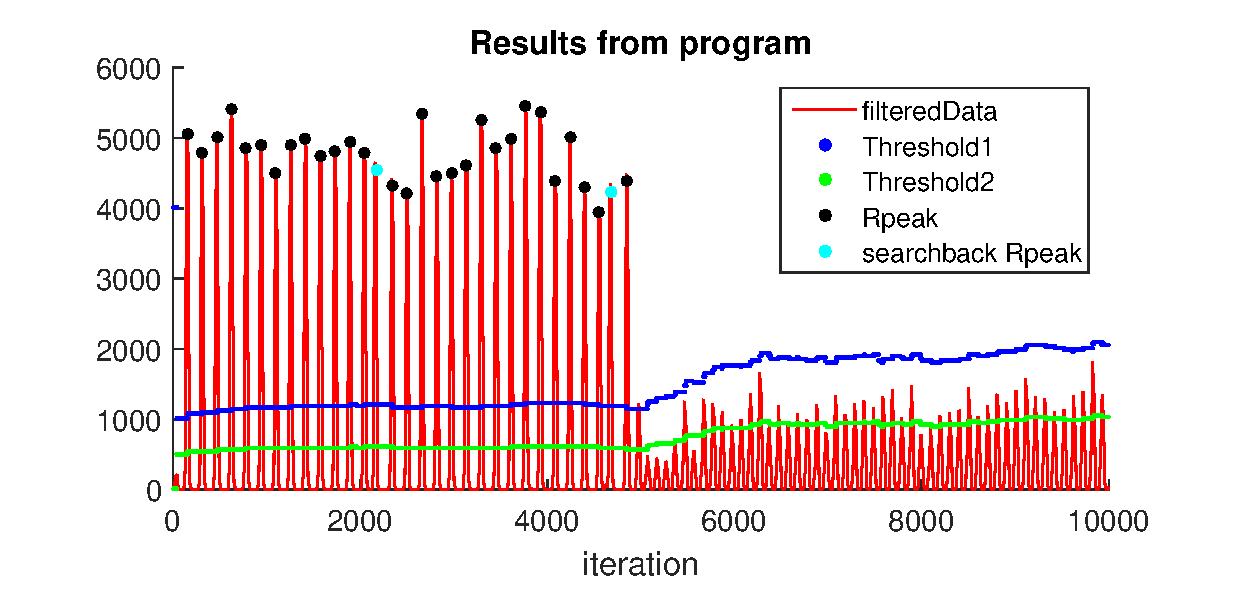
\includegraphics[width=1.0\textwidth]{3Results/fig/10kpointsmatlab.eps}
    \caption{Results from the program, plotted in \texttt{MATLAB}. The thresholds automatically adjust to ignore the noise peaks following the heart failure at iteration $\approx$ 5000. 31 peaks are found (blue, black), 2 of them through searchback (black). }
    \label{fig:10k_points}
\end{figure}

For the first 5000 data points we see that we find Rpeaks and our thresholds are acceptable. Two peaks are found during searchback, at around iteration 2100 and 4500. This would suggest that the peaks come either faster or slower than expected; missing the \texttt{RR\_LOW} to \texttt{RR\_HIGH} interval. After 5000 data points the heartbeat gets alarmingly weak and the thresholds are adjusted. This adjustment is caused by the program recognizing the signal as noise and not accepting the input as Rpeaks.\\
\\
If we look closer in at around iteration 5000 we get figure \ref{fig:1kpoints}.

\begin{figure}[H]
    \centering
    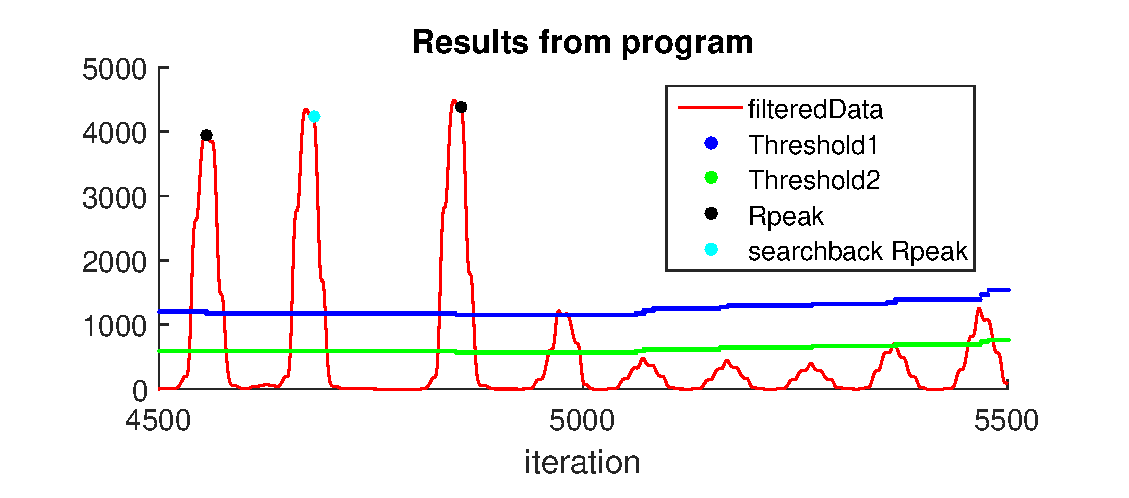
\includegraphics[width=1.0\textwidth]{3Results/fig/1kpointsmatlab.eps}
    \caption{Results from the program, where the peaks found correspond to (local) maxima in the filtered data. If a peak in the filtered data has two smaller peaks, the searchback function finds the latest, i.e. the subpeak at the highest iteration.}
    \label{fig:1kpoints}
\end{figure}

In figure \ref{fig:1kpoints} we see the position of the Rpeak, and how under normal conditions the program detects the first peak (main peak) but in searchback it detects the second peak (subpeak). When the algorithm begins searchback, a new peak stronger than \texttt{THRESHOLD1} must be found first (see figure \ref{fig:QRS_flowchart}). After searchback is executed, the peak (at which the program began searchback from) is ignored, and the next peak found is the subpeak. This results in the subpeak being stored as Rpeak after every searchback, as seen on figure \ref{fig:10k_points}.\\ Figure \ref{fig:1kpoints} shows how the filters has minimized noise between peaks.\\
\\
In figure \ref{fig:comparing_peaks}, we compare our data with the expected output\footnote{The expected output is generated by Nicolai Pedersen, project supervisor.}. we see a clear resemblance, with an average error of 0.4 $\%$, and a maximum error of 4.5 $\%$. Implementations of the filters are known to be different from the expected program structure to our program structure. Our implementation postpones integer division to minimize division error. The differences in results are also at different iterations suggesting that the error is caused by finding different peaks (main peak vs. subpeak).

\begin{figure}[H]
    \centering
    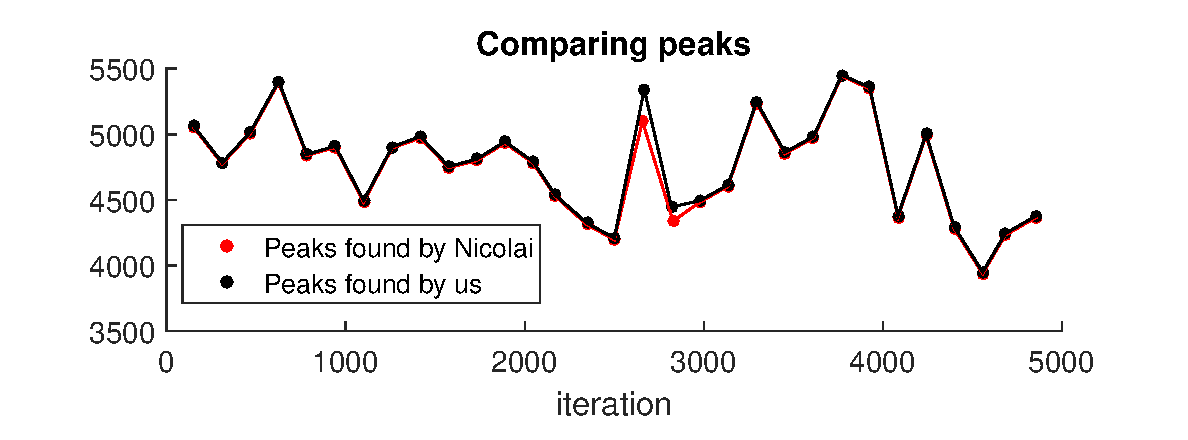
\includegraphics[width=1.0\textwidth]{3Results/fig/comparingPeaks.eps}
    \caption{When comparing our 31 peaks found to those found by Nicolai Pedersen, there is an overall resemblance. The mean absolute difference between red and blue peaks is 0.4 $\%$. The largest different (4.5 $\%$) occurs at iteration 2667. We connected the points to make the graph faster to read.}
    \label{fig:comparing_peaks}
\end{figure}

\subsection{Performance}
\subsubsection{Run-time}
In order to analyze the program performance, several time measurements are performed. \\
\\
Measurement \#1: The time it takes to scan all data points individually from \texttt{ECG.txt}, and store the value in \texttt{originalArray} without any further analysis. The average time of 1000 runs for scanning data is 0.001166 s $=$ 1.17 ms. \\
\\
Measurement \#2: How long it takes to scan all data points and filter the data. The average time of 1000 runs is 0.006607 s $=$ 6.61 ms. Data filtering takes 6.61 ms $-$ 1.17 ms $=$ 5.44 ms. \\
\\
Measurement \#3: The time of scanning data points, filtering data and performing peak detection. The average time of 1000 runs is 0.006626 s $=$ 6.63 ms. Peak detection takes 6.63 ms $-$ 6.61 ms $=$ 0.02 ms.\\
\\
Measurement \#4: The time of scanning data points, filtering data, performing peak detection and outputting data to the user. The average time of 1000 runs is 0.008218 s $=$ 8.22 ms. Printing data to the user takes 8.22 ms $-$ 6.63 ms $=$ 1.59 ms.\\
\\

\begin{table}[H]
\centering
    \label{tab:performance_time}
    \begin{tabular}{ccccc}
    \hline
\multicolumn{1}{|c|}{} & \multicolumn{1}{c|}{\begin{tabular}[c]{@{}c@{}}Scan \\ data points\end{tabular}} & \multicolumn{1}{c|}{\begin{tabular}[c]{@{}c@{}}Filter \\ data points\end{tabular}} & \multicolumn{1}{c|}{\begin{tabular}[c]{@{}c@{}}Peak\\ detection\end{tabular}} & \multicolumn{1}{c|}{\begin{tabular}[c]{@{}c@{}}Print info\\ to user\end{tabular}} \\ \hline
\multicolumn{1}{|c|}{Time (ms)} & \multicolumn{1}{c|}{1.17} & \multicolumn{1}{c|}{5.44} & \multicolumn{1}{c|}{0.02} & \multicolumn{1}{c|}{1.59} \\ \hline
\multicolumn{1}{|c|}{Runtime \%} & \multicolumn{1}{c|}{14.2} & \multicolumn{1}{c|}{66.2} & \multicolumn{1}{c|}{0.002} & \multicolumn{1}{c|}{19.3} \\ \hline                          
    \end{tabular}
\caption{Runtime values and percentages for different program segments}
\end{table}


This clearly shows that the filtering is the slowest part of the program, and that it would be reasonable to move data filtering to the hardware (and optimize filtering functions). Peak detection is remarkably quick. This is understandable: the main part of peak detection is only run if a peak is found. Otherwise it only performs one comparison and increments a counter.

\subsubsection{Energy consumption}
These time measurements are performed on a MacBook pro on a 2.7 GHz Intel Core i5 processor with a 35 W TDP divided on two cores, resulting in a complete energy consumption of 8.22 ms $\cdot$ 35 W$\cdot \frac{1}{2}=$ 0.15 J for the complete data set. 

\section{Conclusion}
We have successfully implemented the QRS algorithm in C. Data acquisition, data filtering and peak detection are handled much faster than the data is produced in real-time. The C code is relatively small (in the order of KB), and the program has relatively low energy consumption. Hence we determine that it is indeed reasonable to implement the algorithm in an embedded system.

\subsection{Discussion}
When implementing the QRS algorithm, we realized an ambiguity in the flowchart supplied by the assignment. When the \texttt{searchback} function found a peak (peak2), the current RR value is the interval from the previous Rpeak to the next peak stronger than \texttt{THRESHOLD1}. This RR value is \underline{not} the peak stored in \texttt{Rpeak}.

Every time an average is calculated (in moving window integration filter, \texttt{RecentRR} and \texttt{RecentRR\_OK}) the array is summed and divided by the number of elements. This is a resource-heavy computation. A more elegant implementation would be to update the average (a sum) with only two calculations: Adding the difference between the new and oldest values, divided by the number of elements averaged over. Example:

\begin{lstlisting}
sum = sum + (newElement - oldestElement)/N;
\end{lstlisting}

One of the best decisions during this project was to put all data in \texttt{data} and use pointers as function parameters, minimizing data transfer and maximizing accessibility. 

\subsection{Which parts of the program be implemented in hardware?}
We expect that the data filtering can be implemented in hardware. The filtering uses integer addition and integer multiplication, and several numbers (for independent filters) be calculated simultaneously. 

% send filer: c og h
% hvis projekt: check image


\newpage
\section{Appendix}

\subsection{Appendix A. How the filters alter the signal}
\label{Apx:A}

\begin{figure}[H]
    \centering
    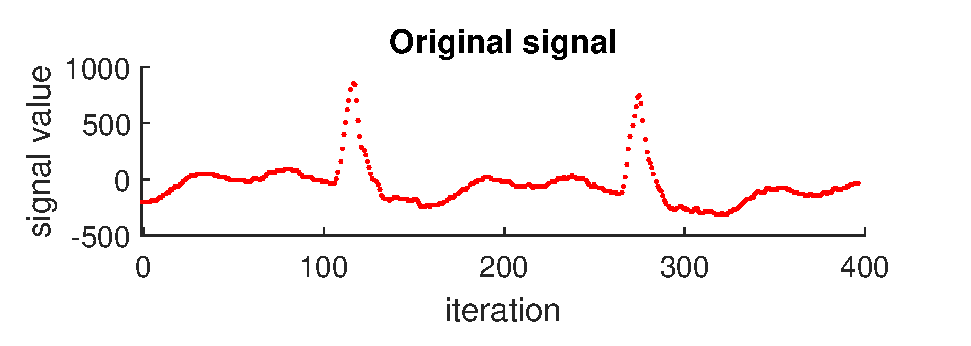
\includegraphics[width=1.0\textwidth]{Appendix/fig/1original.eps}
    \caption{Signal as a function of iteration.}
    \label{fig:1original}
\end{figure}

\begin{figure}[H]
    \centering
    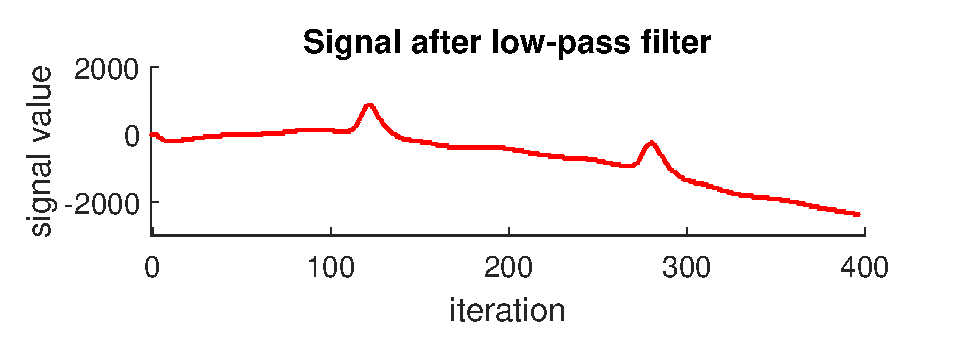
\includegraphics[width=1.0\textwidth]{Appendix/fig/2afterLowPass.eps}
    \caption{Signal as a function of iteration.}
    \label{fig:2afterLowPass}
\end{figure}

\begin{figure}[H]
    \centering
    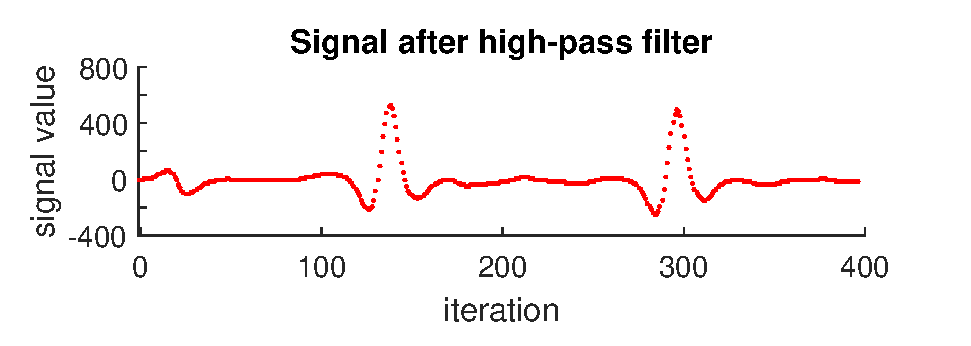
\includegraphics[width=1.0\textwidth]{Appendix/fig/3afterHighPass.eps}
    \caption{Signal as a function of iteration.}
    \label{fig:3afterHighPass}
\end{figure}

\begin{figure}[H]
    \centering
    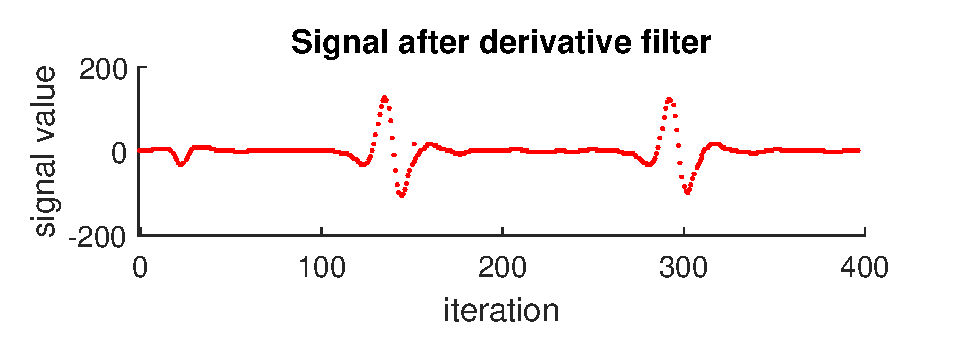
\includegraphics[width=1.0\textwidth]{Appendix/fig/4afterDerivative.eps}
    \caption{Signal as a function of iteration.}
    \label{fig:4afterDerivative}
\end{figure}

\begin{figure}[H]
    \centering
    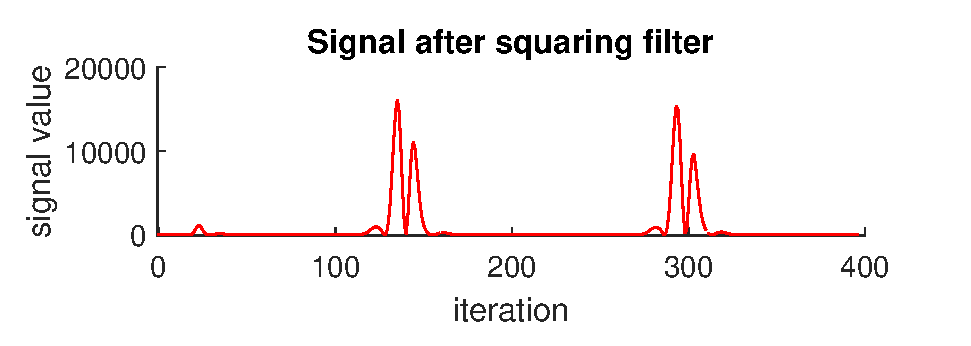
\includegraphics[width=1.0\textwidth]{Appendix/fig/5afterSquaring.eps}
    \caption{Signal as a function of iteration.}
    \label{fig:5afterSquaring}
\end{figure}


\begin{figure}[H]
    \centering
    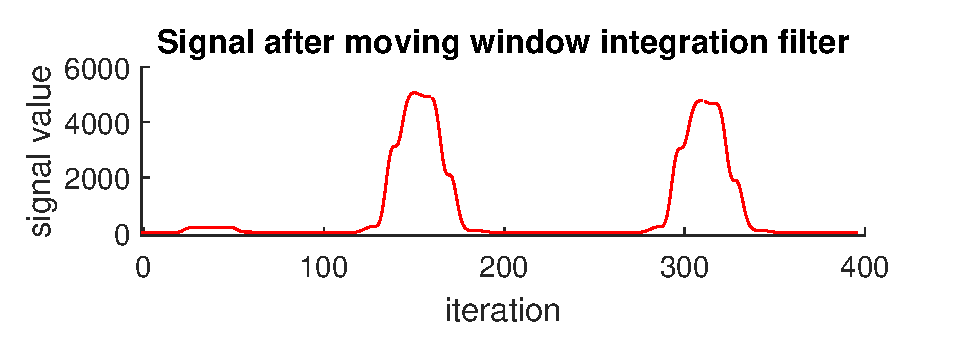
\includegraphics[width=1.0\textwidth]{Appendix/fig/6afterMovInt.eps}
    \caption{Signal as a function of iteration.}
    \label{fig:6afterMovInt}
\end{figure}



\newpage
\subsection{Appendix B: struct DATA data}
\label{Apx:B}
\begin{multicols}{2}

\begin{lstlisting}
typedef struct DATA{
// stores all variables
    
    // ints
    int peakCheck;
    int lastCheck;
    int peakValue;
    int bpm;
    int iteration;
    int lastRpeakTime;
    int missIntervalCounter;
    int RR;
    int RpeakCounter;
    int lastPeak;
    int peak2;
    
    // doubles for peak detection
    double SPKF;
    double NPKF;
    double THRESHOLD1;
    double THRESHOLD2;
    double RR_AVERAGE1;
    double RR_AVERAGE2;
    double RR_LOW;
    double RR_HIGH;
    double RR_MISS;

    // arrays for QRS algorithm, and data
    int RecentRR[8];
    int RecentRR_OK[8];
    int peaks[ARRAY_LENGTH];
    int peakTimeStamps[ARRAY_LENGTH];
    int Rpeak [ARRAY_LENGTH];
    int originalArray[ARRAY_LENGTH];
    int afterLowPass[ARRAY_LENGTH];
    int afterHighPass[ARRAY_LENGTH];
    int afterDerivAndSquare[ARRAY_LENGTH];
    int filteredData[ARRAY_LENGTH];
    
    // pointer to .txt file
    FILE *fp;
    
} DATA;
\end{lstlisting}

\end{multicols}







\end{document}

